\chapter{Diagrammes de classes}

Cette partie contient tous les diagrammes de classes décrivant l'architecture du site web. Certains diagrammes peuvent être aussi accompagné des quelques explications.

\newpage

\section{Diagrammes de classes de l'application cakephp}

\subsection{Contrôleurs}

\begin{figure}[H]
	\begin{center}\fbox{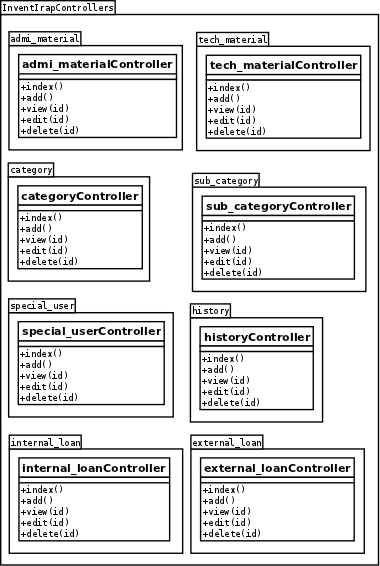
\includegraphics[]{images/controller.png}}\end{center}
	\caption{Contrôleurs du site web}
\end{figure}

\subsection{View}

\begin{figure}[H]
	\begin{center}\fbox{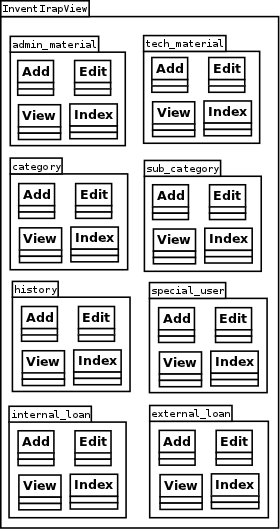
\includegraphics[]{images/view.png}}\end{center}
	\caption{Vues du site web}
\end{figure}

Les classes définies dans ce diagramme sont en fait des fichier .cpt qui ne représentent que de simples fichiers php.
